\graphicspath{{{media/}}}
\section{Zahlenfolgen}
In diesem Kapitel geht es – wie der Titel schon sagt – um Zahlenfolgen.
Mit ihnen lassen sich besonders gut Prozesse beschreiben, bei denen sich eine Grösse schrittweise verändert.
Zum Schluss des Kapitels werden auch erste Überlegungen zur «Infinitesimalrechnung» gemacht, 
bei der es um den Umgang mit dem Begriff «unendlich» geht. Dabei werden unendlich lange Prozesse
betrachten und eine Technik aufgezeigt, diese gewissermassen «zu Ende zu denken».
%Ausserdem wird eine ganz wichtige neue Beweismethode vorgestellt, bei der man unendliche viele Aussagen gleichzeitig beweisen kann.
 

\subsection{Folgen und Reihen allgemein}
Beginen wir mit einer berühmten Überlegung,
bei der es um die Entwicklung einer Kaninchen-Population geht:
\begin{LA} {Einführung}{}
    Der italienische Mathematiker Leonardo da Pisa genannt Fibonacci
    hat im Jahr 1202 ein Modell für das Wachstum einer Kaninchenpopulation erstellt.
    Dazu hat er die folgenden vereinfachenden Annahmen getroffen:
    \begin{itemize}
        \item Die Beobachtung beginnt mit einem neugeborenen Kaninchenpaar.
        \item Jedes neugeborene Kaninchenpaar wird nach zwei Monaten geschlechtsreif.
        \item Jedes geschlechtsreife Kaninchenpaar bringt jeden Monat ein neues Kaninchenpaar zur Welt.
        \item Im beobachteten Zeitraum sterben keine Kaninchen.
    \end{itemize}
    Füllen Sie die Tabelle unten aus.
    Wie gross ist nach diesem Modell die Anzahl Kaninchenpaare $a_n$ nach Ablauf von $n$ Monate?
    
    \begin{center}
        \begin{tabular}{c|c|c|l}
            Nach Monate& unreife Paare  & reife Paare &  Total Paare  \\ \hline
            1& 1 & 0 &  $a_1 = 1$  \\
            2& 0 & 1 &  $a_2 = 1$  \\
            3& 1 & 1 &  $a_3 = 2$  \\ &&&\\
            4&  &  &  $a_4 = $  \\ &&&\\
            5&  &  &  $a_5 =  $  \\ &&&\\
            6&  &  &  $a_6 =  $  \\ &&&\\
            7&  &  &  $a_7 =  $  \\ &&&\\
            8&  &  &  $a_8 =  $  \\
        \end{tabular} 
    \end{center}
 
        Können Sie eine Rechenvorschrift angeben, mit der man die Anzahl Kaninchenpaare nach $n$ Monate berechnen kann?
\end{LA}
\subsubsection{Rekursive und explizite Definitionen}
\begin{bsp}{Erste Folgen}{ersteFolgen}
    In der Regel werden Folgen mit $(a_n)_{n\in \N}$ gekennzeichnet oder einem anderen passenderen Buchstaben.
    \begin{itemize}
        \item Die Folge $(a_n)_{n\in \N}$ der Zweierpotenzen: \[2, 4, 8, \cdots\]
            In diesem Fall bezeichnet $a_1 = 2$ das erste Folgenglied und $a_5=32$ das fünfte.
        \item Die Folge $(b_n)_{n\in \N}$ der ungeraden Zahlen: \[1, 3, 5, \cdots\]
        In diesem Fall bezeichnet $b_1 = 1$ das erste Folgenglied und $b_7=13$ das siebte.
        \item Die Fibonacci Folge $(f_n)_{n\in \N}$: \[1, 1, 2, 3, 5, \cdots\]
        \item Die Folge der Primzahlen $(p_n)_{n\in \N}$: \[2, 3, 5, 7, 11, \cdots\]
    \end{itemize}
\end{bsp}

Unter der Definition einer Folge versteht man eine Rechenvorschrift, mit der man 
jedes  Glied einer Folge bestimmen kann. Bei Folgen werden Grundsätzlich zwei Arten von Definitionen unterschieden:

\begin{definition}{Rekursive und explizite Definitionen}{}
    Eine \emph{rekursive Definition} einer Folge ist eine Rechenvorschrift, mit der man ein Folgenglied aus den vorhergehenden berechnen kann. Dabei muss mindestens ein konkretes Folgeglied angegeben werden (häufig das erste Glied der Folge).

    Eine \emph{explizite Definition} einer Folge ist eine Rechenvorschrift, mit der man jedes Folgenglied direkt berechnen kann – ohne Kenntnis von anderen Folgengliedern.

\end{definition}

Die Folgen im \Cref{bsp:ersteFolgen}, können wie folgt auf die beiden Arten definiert werden:
\begin{itemize}
    \item Zweierpotenzen:
    
    \emph{rekursive Definition:} 
    \vspace*{1cm}
    %\vfill
    
    % das erste Glied der Folge ist $a_1=2$.
    % Für alle $n>1$ gilt \newline
    % $a_n=2\cdot a_{n-1}, \quad a_1=2$  (Alternativ auch $a_{n+1}=2\cdot a_n$, für alle $n\ge 1$)
    
    \emph{explizite Definition:} %$a_n=2^n$ für alle $n\in \N$
    \vspace*{1cm}
    %\vfill
    \newpage
    \item 	Ungerade Zahlen:
    
    \emph{rekursive Definition:}  %$b_1=1,b_n=b_{n-1}+2$ für alle $n>1$.
    \vspace*{1cm}
    %\vfill

    \emph{explizite Definition:}  %$b_n=2n-1$ für alle $n\in \N$.
    \vspace*{1cm}
    %\vfill

    \item 	Fibonacci-Folge:
    
    \emph{rekursive Definition}: %$f_1=1,f_2=1$ und $f_n=f_{n-1}+f_{n-2}$ für alle $n>2$.
    \vspace*{1cm}

    \emph{explizite Definition} 
    %     von de Moivre (1730, also 500 Jahre nach Fibonacci!)
    % $$
    % f_n=\frac{1}{\sqrt{5}}  \left[ \left( \frac{1+\sqrt 5}{2} \right)^n - \left( \frac{1-\sqrt 5}{2} \right)^n \right] $$
    \vspace*{1cm}
    %\vfill

    \item \emph{Primzahlfolge:} %unbekannt!
    \vspace*{1cm}
    %\vfill

\end{itemize}

%\clearpage
\begin{bsp}
    {Wie berechnet man z. B. das 4. Glied einer Folge?}{}
   
    \begin{itemize}
         
        \item 	Wenn die Folge explizit definiert ist,
         z.B. $a_n=\frac{3}{n}$ ist es ganz einfach. Man muss bloss $n=4$ einsetzen:
          $a_4=\frac{3}{4}$.
        \item 	Wenn die Folge rekursiv definiert ist, z.B. $a_{n+1}= 2a_n + 3, a_1=-1$,
        muss man der Reihe nach für $n$ die Zahlen $1,2$ und $3$ einsetzen: \newline
        $n=1$ liefert: $a_{1+1}=2a_1+3$ also $a_2=2\cdot (-1)+3=1$  \newline
        $n=2$ liefert: $a_{2+1}=2a_2+3$ also $a_3=2\cdot 1+3=5$  \newline
        $n=3$ liefert: $a_{3+1}=2a_3+3$ also $a_4=2\cdot 5+3=13$ 
        
    \end{itemize}
\end{bsp}
Man kann Zahlenfolgen übrigens auch als eine besondere Klasse von Funktionen betrachten.
Dabei spielt die Zahl $n$ die Rolle des Inputs und der entsprechende Output ist dann das Folgeglied $a_n$.
Speziell ist, dass nur natürliche Zahlen als Inputs zugelassen sind. In der formalen Sprache der Mathematik kann das so ausgedrückt werden:
$$ \N \rightarrow \R, \quad n \mapsto a_n $$
Der Definitionsbereich ist $\N$, die Wertemenge ist $\R$ und der Funktionswert an der Stelle $n$ ist $a_n$.

\pagebreak
\begin{ueb}{Zu rekursiver und expliziter Definition}{rek&expliziteDef}
    %% Die Auskommentierten sind die anderen Aufgaben aus Rhyn
    %% Vor dem Einsatz müsste man die Zahlen kontrollieren
    \begin{enumerate}
        \item Berechne die ersten fünf Glieder der gegebenen Folge $n \mapsto a_n$.
        \begin{enumerate}
            %\item $a_n = 3n$
            \item $a_n = 4n - 1$
            % \item $a_n = \frac{2n}{n+3}$
            % \item $a_n = n^2 + 3$
            % \item $a_n = \frac{n}{n^2 - 2}$
            \item $a_n = 2^{3-n}$
            % \item $a_n = (-1)^n$
            \item $a_n = n + (-1)^n$
            \item $a_n = 5 + 2(-1)^n$
        \end{enumerate}
    
        % \item Ergänze jeweils auf die ersten sieben Glieder der Folge.
        % \begin{enumerate}
        %     \item $a_1 = 5, \quad a_2 = -2, \quad a_3 = -9$
        %     \item $a_3 = \frac{7}{4}, \quad a_4 = \frac{9}{8}, \quad a_5 = \frac{11}{16}$
        %     \item $a_2 = 25, \quad a_4 = 49, \quad a_5 = 64$
        %     \item $a_4 = 6, \quad a_5 = 3, \quad a_6 = 1.5$
        %     \item $a_3 = \frac{9}{34}, \quad a_4 = \frac{16}{39}, \quad a_5 = \frac{49}{54}$
        %     \item $a_2 = \frac{5}{8}, \quad a_3 = \frac{13}{21}, \quad a_4 = \frac{34}{55}$
        % \end{enumerate}
    
        \item Bestimme das allgemeine Glied $a_n$ der Folge. Hierfür gibt es kein `Rezept'.
        Versuchen Sie, ein Muster zu erkennen und es in Form einer expliziten Definition der Folge anzugeben. (Wenn Sie es eine Weile lang nicht erkennen, blicken Sie in die Lösungen)
        \begin{enumerate}
            \item $4, 8, 12, \dots$
            \item $3, 5, 7, \dots$
            % \item $16, 21, 26, \dots$
            % \item $2, 4, 8, 16, \dots$
            % \item $1, \frac{1}{2}, \frac{1}{4}, \dots$
            % \item $\frac{2}{4}, \frac{9}{13}, \frac{6}{17}, \dots$
            % \item $1, -1, 1, -1, \dots$
            \item $2, 0, 2, 0, 2, 0\dots$
            
        % \end{enumerate}
    
        % \item Ebenso.
        % \begin{enumerate}
            % \item $0, -2, -4, -6, \dots$
            % \item $-7, -3, 1, 5, \dots$
            \item $0, 1, 4, 9, 16, \dots$
            \item $0, \frac{1}{2}, \frac{2}{3}, \frac{3}{4}, \dots$
            %\item $-\frac{1}{8}, -\frac{4}{27}, -\frac{9}{64}, -\frac{16}{125}, \dots$
            \item $-5, 1, -5, 1, -5, \dots$
            \item $-\frac{3}{5}, \frac{11}{13}, -\frac{19}{21}, \frac{27}{29} \dots$
            %\item $2, 6, 12, 20, 30, \dots$
        \end{enumerate}
    
        \item Bestimme die ersten fünf Glieder der rekursiv definierten Folge.
        \begin{enumerate}
            \item $a_1 = 20, \quad a_{n} = a_{n-1} - 4$
            \item $a_1 = 1, \quad a_{n+1} = 3 a_n$
            \item $a_1 = 1, \quad a_{n} = 2 a_{n-1} + 3$
            \item $a_1 = 0, \quad a_{n+1} = a_n + \frac{2}{(n+2)(n+3)}$
            % \item $a_1 = 1, \quad a_{n+1} = 2 a_n - 3$
            % \item $a_1 = 0, \quad a_{n+1} = 3 a_n + 3^n$
            % \item $a_1 = a_2 = 1, \quad a_{n+2} = a_n + a_{n+1}$
            % \item $a_1 = 2, \quad a_2 = 1, \quad a_{n+2} = a_n \cdot a_{n+1} - n$
        \end{enumerate}
    
        \item Geben Sie die explizite Definition der Folgen aus Aufgabe 3 an.
        \item Definiere die Folge durch eine Rekursionsformel.
        \begin{enumerate}
            \item $50, 47, 44, 41, \dots$
            \item $3, 6, 12, 24, \dots$
            \item $2, 3, 5, 8, 12, \dots$
            % \item $5, 9, 17, 33, 65, \dots$
            % \item $1, 4, 10, 19, 31, \dots$
            % \item $4, 10, 22, 46, 94, \dots$
        \end{enumerate}
    \end{enumerate}
    



    % Alle Übungen zum Thema Analysis entnehmen Sie dem Aufgabenbuch «Analysis» von Erhard Rhyn.
    % Zu jeder Aufgabe gibt es im Buch Kurzlösungen.
    % Sie finden sie ab Seite 61 im Buch. Die Zahl im grauen Kästchen gibt an, auf welches Seite sich die entsprechenden Aufgaben befinden.
    % %Siehe Bild.
    % %\includegraphics{rhynloesg.jpg}

    % Machen Sie sich mit den Zahlenfolgen vertraut, indem Sie die folgenden Übungen lösen.
    % \begin{itemize}
    %     \item 1b) f) und h)
    %     \item 3a) b) und h) hierfür gibt es kein Rezept.
    %     Versuchen Sie, ein Muster zu erkennen und es in Form einer expliziten Definition der Folge anzugeben. (Wenn Sie es eine Weile lang nicht erkennen, blicken Sie in die Lösungen)
    %     \item 3i) als freiwillige Challenge
    %     \item 4c)d)h) gehen Sie vor wie bei Aufgabe 3
    %     \item 5a)c)d) und h) Achtung bei d): um das Glied $a_2$  zu bestimmen, muss man in der Rekursionsgleichung $n=1$ einsetzen...
    %     \item 6a)c)d)
    %     \item 7a)b)c) wie bei 3, aber mit einer rekursiven Definition
    % \end{itemize}
\end{ueb}
\clearpage
\begin{ueb}
    {Bonus: Programmieraufgabe}{}
    Es bietet sich an, Folgenglieder mit einem kleinen Programm zu berechnen.

    Das nachfolgende Programm löst die Aufgabe 1(a) aus \Cref{uebng:rek&expliziteDef}:

    \lstinputlisting[language=Python]{Folgenrechner.py}

    Es lassen sich auch rekursiv definierte Folgen berechnen. Dazu verwendet man eine Funktion, die sich selbst aufruft. Betrachten Sie dazu der folgende Programmcode, der die Aufgabe 3(a) aus \Cref{uebng:rek&expliziteDef} löst. 

    \lstinputlisting[language=Python]{folgenrechnerRek.py}

    Passen Sie die Programme an und lösen Sie damit die anderen Teilfragen von Aufgabe 1 und 3 aus \Cref{uebng:rek&expliziteDef}.
\end{ueb}












\clearpage
\emph{Lösungen}
\begin{enumerate}
    \item Berechne die ersten fünf Glieder der gegebenen Folge $n \mapsto a_n$.
    \begin{enumerate}
        \item $a_n = 4n - 1$: \quad $3, 7, 11, 15, 19$
        \item $a_n = 2^{3-n}$: \quad $4, 2, 1, \frac{1}{2}, \frac{1}{4}$
        \item $a_n = n + (-1)^n$: \quad $0, 3, 2, 5, 4$
        \item $a_n = 5 + 2(-1)^n$: \quad $3, 7, 3, 7, 3$
    \end{enumerate}

    \item Bestimme das allgemeine Glied $a_n$ der Folge.
    \begin{enumerate}
        \item $a_n = 4n$
        \item $a_n = 2n + 1$
        \item $a_n = 1 - (-1)^n$
        \item $a_n = (n-1)^2$
        \item $a_n = \frac{n-1}{n}$
        \item $a_n = -2 + 3(-1)^n$
        \item $a_n = (-1)^n \cdot \frac{8n-5}{8n-3}$
    \end{enumerate}

    \item Bestimme die ersten fünf Glieder der rekursiv definierten Folge.
    \begin{enumerate}
        \item $a_1 = 20, a_{n+1} = a_n - 4$: \quad $20, 16, 12, 8, 4$
        \item $a_1 = 1, a_{n+1} = 3 a_n$: \quad $1, 3, 9, 27, 81$
        \item $a_1 = 1, a_{n+1} = 2 a_n + 3$: \quad $1, 5, 13, 29, 61$
        \item $a_1 = 0, a_{n+1} = a_n + \frac{2}{(n+2)(n+3)}$: \quad $0, \frac{1}{6}, \frac{4}{15}, \frac{1}{3}, \frac{8}{21}$
    \end{enumerate}

    \item Geben Sie die explizite Definition der Folgen aus Aufgabe 3 an.
    \begin{enumerate}
        \item $a_n = 24 - 4n$
        \item $a_n = 3^{n-1}$
        \item $a_n =2^{n+1}-3$
        \item $a_n =\frac{2 (n-1)}{3(n+2)}$ (Tipp: Es ist einfacher, wenn man die Brüche nicht kürzt) 
    \end{enumerate}

    \item Definiere die Folge durch eine Rekursionsformel.
    \begin{enumerate}
        \item $a_1 = 50, a_{n+1} = a_n - 3 $
        \item $a_1 = 3, a_{n+1} = 2\cdot a_n $
        \item $a_1 = 2, a_{n+1} = a_n + n $
        % \item $a_1 = 5, a_{n+1} = 2\cdot a_n -1 $
        % \item $a_1 = 1, a_{n+1} = a_n + 3n $
        % \item $a_1 = 4, a_{n+1} = 2a_n + 2 $
    \end{enumerate}
\end{enumerate}









\clearpage
\subsubsection{Reihen und Summenzeichen}
\begin{LA}
    {Einführung}{E-in-Reihen.}
    Was passiert, wenn man die Glieder einer Folge aufsummiert? Untersuchen Sie dazu die folgenden Beispiele
    \begin{enumerate}
        \item Gegeben ist die Folge $a_n$ der ungeraden Zahlen $1, 3, 5, 7, 9, \dots $.

        Berechnen Sie die Summen $s_1=a_1,\  s_2 = a_1+a_2,\  s_3=a_1+a_2+a_3, \dots$.

        Was vermuten Sie: Wie gross ist $s_{100} = a_1+a_2+a_3 + \cdots + a_{100}$?
        \item Gegeben ist die Folge $1, -2, 3, -4, 5, \dots $. Berechnen Sie wieder die Summen $s_1, s_2, s_3 \dots$. Wie gross ist $s_{100}$ in diesem Fall?
        \item Beantworten Sie die gleiche Frage für die Folge der Zweierpotenzen $1, 2, 4, 8, 16, \dots$.
    \end{enumerate}
\end{LA}

\clearpage
Ausgehend von einer Zahlenfolge kann man eine dazugehörige Reihe definieren. Dabei handelt es sich wiederum um eine Zahlenfolge:
\begin{definition}
    {Reihen und Partialsumme}{Reihe}
Gegeben eine Folge $a_1,a_2,\dots $. Werden die ersten $n$ Glieder der Folge aufsummiert, so erhalten wir die sogenannte \emph{Partialsumme} $s_n$:
$$ s_n = a_1+a_2+a_3 + \cdots + a_{n}$$

Die Partialsummen $s_1,s_2,\dots$ bilden selbst wieder eine Zahlenfolge, die sogenannte \emph{Partialsummenfolge} oder \emph{Reihe}.

Die Folge $(s_n)$ kann rekursiv definiert werden durch:
$$s_1=a_1,\quad  s_{n+1}=s_n + a_{n+1} $$


\end{definition}

\begin{bsp}
    {Reihe zur Folge der Zweierpotenzen}{ReiheZweierpotenz}
    Die zur Folge der Zweierpotenzen $1, 2, 4, 8, 16, \dots$ gehörende Reihe ist


    \vspace*{3cm}
\end{bsp}

Für das Aufsummieren von Folgenglieder wird häufig das Summenzeichen $\Sigma$ verwendet. Dieses versteht man am einfachsten anhand eines Beispiels: $\sum_{k=3}^{7} (3k-1)$ ist die Summe aller Glieder der Folge $a_k=3k-1$, wobei $k$ bei $3$ beginnt und alle ganzen Zahlen bis und mit $7$ durchläuft. Also
$$\sum_{k=3}^{7} (3k-1) = (3\cdot 3 -1)+ (3\cdot 4 -1)+ (3\cdot 5 -1)+ (3\cdot 6 -1)+ (3\cdot 7 -1)=70$$



\begin{definition}
    {Summenzeichen $\Sigma$}{}
    Der Ausdruck  $ \sum\limits_{k=m}^{n} a_k$ bezeichnet die Summe aller Glieder der Folge $a_k$ beginnend mit $k=m$ bis $k=n$, Grenzen inklusive.

    Anstatt $k$ kann auch eine andere Variable verwendet werden. (Häufig $i, j$ oder $n$)
\end{definition}
\clearpage
\begin{ueb}
{Zu Reihen und Summenzeichen}{ReiheSumme}
\begin{enumerate}
\item Die Folge ist durch das allgemeine Glied $a_k = 2k+10$ gegeben. Notiere die dazugehörige Partialsummen ohne Summenzeichen und rechne sie aus.
\begin{enumerate}
    \item $\sum\limits_{k=1}^{4} a_k$
    \item $\sum\limits_{k=5}^{7} a_k$
    \item $\sum\limits_{k=1}^{7} a_k$
    \item $\sum\limits_{k=1}^{4} (2\cdot a_k)$
\end{enumerate}

\item Notiere die Summe mit dem Summenzeichen $\sum$. Die Summe muss nicht ausgerechnet werden.
    \begin{enumerate}
        \item $5 + 10 + 15 + 20 + 25 + 30 + 35$
        \item $5 + 10 + 15 + 20 + \dots + 250$
        \item $25 + 30 + 35 + 40 + \dots + 105$
        \item $3 + 9 + 27 + 81 + 243$
        \item $1 + 4 + 9 + 16 + \dots + 400$
        \item $0 + 3 + 6 + 9 + 12 + \dots + 345$
    \end{enumerate}
\item Teleskopsummen: Von einer Folge ist das allgemeine Glied $a_k$ gegeben und $s_n$ bezeichnet ihre $n$-te Partialsumme.
\begin{enumerate}
    \item Berechne $s_3$ und $s_8$ für $a_k = \sqrt{k+1} - \sqrt{k}$ und stelle $s_n$ als vereinfachten Term dar.
    \item Berechne $s_4$ und $s_9$ für $a_k = \frac{1}{k^2} - \frac{1}{(k+1)^2}$ und stelle $s_n$ als vereinfachten Term dar.
    \item Berechne $s_{15}$ für $a_k = \frac{1}{\sqrt{k}} - \frac{1}{\sqrt{k+1}}$ und stelle $s_n$ als vereinfachten Term dar.
    \item Challenge: Berechnen Sie $s_{99}$ für die Folge $a_k = \log\left(\frac{k+1}{k}\right)$.
\end{enumerate}
\end{enumerate}
\end{ueb}
\clearpage
\begin{ueb}
    {Bonus: Programmieraufgabe}{}
    Wieder bietet sich an, die Berechnung der Reihenglieder mit einem kleinen Programm durchzuführen.

    Das nachfolgende Programm berechnet die ersten fünf Glieder der Reihe $s_n = \sum\limits_{k=1}^n 2^{k-1}$, die zur Folge der Zweierpotenzen gehört (Siehe \Cref{bsp:ReiheZweierpotenz} )

    \lstinputlisting[language=Python]{Reihenrechner.py}

    \begin{enumerate}
        \item Passen Sie das Programm an, um damit die Aufgabe 3 aus \Cref{uebng:ReiheSumme} zu lösen. Für die Wurzeln und den Logarithmus zur Basis 10 müssen Sie die entsprechenden Funktionen aus der math-Bibliothek importieren:
        \begin{lstlisting}[language=Python]
    from math import log10, sqrt     \end{lstlisting}
    \item Für die Berechnung der Reihenglieder könnte man auch die rekursive Definition $s_1=a_1,\quad  s_{n+1}=s_n + a_{n+1} $ verwenden. Passen Sie die Funktion s(n) im Programm entsprechend an.
        
    \end{enumerate}
    
\end{ueb}




\clearpage
\emph{Lösungen}
\begin{enumerate}
    \item Die Folge ist durch das allgemeine Glied $a_k = 2k+10$ gegeben. Notiere die dazugehörige Partialsummen ohne Summenzeichen und rechne sie aus.
    \begin{enumerate}
        \item $\sum\limits_{k=1}^{4} a_k = (12 + 14 + 16 + 18) = 60$
        \item $\sum\limits_{k=5}^{7} a_k = (20 + 22 + 24) = 66$
        \item $\sum\limits_{k=1}^{7} a_k = (12 + 14 + 16 + 18 + 20 + 22 + 24) = 60 + 66 = 126$ 
        \item $\sum\limits_{k=1}^{4} (2\cdot a_k) = 24+28+32+36 = 2(12 + 14 + 16 + 18) = 120$
    \end{enumerate}

    \item Notiere die Summe mit dem Summenzeichen $\sum$. Die Summe muss nicht ausgerechnet werden.
    \begin{enumerate}
        \item $\sum\limits_{k=1}^{7} 5k$
        \item $\sum\limits_{k=1}^{50} 5k$
        \item $\sum\limits_{k=5}^{21} 5k$
        \item $\sum\limits_{k=1}^{5} 3^k$
        \item $\sum\limits_{k=1}^{20} k^2$
        \item $\sum\limits_{k=0}^{115} 3k = \sum\limits_{k=1}^{116} (3k -3)= \sum\limits_{k=1}^{116} 3(k -1)$
    \end{enumerate}

    \item Teleskopsummen: Es lassen sich immer alle Summanden bis auf zwei wegstreichen :)
    \begin{enumerate}
        \item $s_3 = \sqrt{4} - \sqrt{1} = 2 - 1 = 1$, \quad $s_8 = \sqrt{9} - \sqrt{1} = 3 - 1 = 2 \quad s_n = \sqrt{n+1} - 1$ 
        \item $s_4 = \frac{1}{1} - \frac{1}{5^5} = \frac{24}{25}$, \quad $s_9 = \frac{99}{100}, \quad s_n = 1-\frac{1}{(n+1)^2}$
        \item $s_{15} = \frac{1}{\sqrt{1}} - \frac{1}{\sqrt{16}} = \frac{3}{4} \quad s_n = 1-\frac{1}{\sqrt{n+1}}$
        \item Mit dem Logarithmus-Gesetz $\log(\frac{a}{b}) = \log a - \log b$ findet man 
        $s_{99} = 2$
    \end{enumerate}
\end{enumerate}

















%%%%%%% Alte Version 2024 %%%%%%%%%%%%%
% \subsubsection{Summenzeichen, monotone und beschränkte Folgen}
% In einigen Aufgaben wird das Summenzeichen $\sum$ verwendet. Das versteht man am einfachsten anhand eines Beispiels:
% $\sum_{k=3}^{7} (3k-1)$ ist die Summe aller Terme der Form $3k-1$, wobei $k$ bei $3$ beginnt und alle ganzen Zahlen bis und mit $7$ durchläuft. Also
% $$\sum_{k=3}^{7} (3k-1) = (3\cdot 3 -1)+ (3\cdot 4 -1)+ (3\cdot 5 -1)+ (3\cdot 6 -1)+ (3\cdot 7 -1)=70$$

% Ausserdem gibt es Folgen mit besonderen Eigenschaften

% \begin{definition}{Monotonie}{}
%     Eine Folge $a_n$ heisst \emph{monoton wachsend} (oder \emph{monoton steigend}), wenn für alle $n\in \N$ gilt
% $$a_{n+1}\ge a_n$$
% Sie heisst \emph{streng monoton wachsend}, wenn für alle $n\in \N$ gilt
% $$a_{n+1} > a_n$$
% Analog gibt es die Begriffe \emph{monoton fallend und streng monoton fallend}.

% \end{definition}

% \begin{definition}{Beschränktheit}{}
%     Eine Folge $a_n$ heisst \emph{nach unten beschränkt},  wenn es eine Zahl $a\in\R$ gibt, sodass für alle $n\in \N$ gilt
%     $$ a_n\ge a $$
%     Eine Folge $a_n$ heisst \emph{nach oben beschränkt},  wenn es eine Zahl $b\in\R$ gibt, sodass für alle $n\in \N$ gilt
%     $$a_n\le b$$
% \end{definition}

% \begin{bsp}
%     {Nachweis von Monotonie und Beschränktheit}{}
%     Behauptung: Die Folge $a_n=\frac{n+1}{n}$ ist monoton fallend, nach unten durch $a=1$ beschränkt und nach oben durch $b=2$.
    
%     \emph{Nachweis der Monotonie:}
%     $$a_{n+1}< a_n \iff \frac{(n+1)+1}{(n+1)} < \frac{n+1}{n} \iff \frac{n+2}{n+1}<\frac{n+1}{n}$$
%     werden beide Seiten der Ungleichung mit der positiven Zahl $n(n+1)$ multipliziert, erhält man die dazu äquivalente Ungleichung
%     $$ n(n+2)<(n+1)^2\iff n^2+2n < n^2+2n+1 \iff 0<1 $$
%     Da die letzte Ungleichung offensichtlich stimmt, muss auch die dazu äquivalente erste Ungleichung $a_{n+1}<a_n$ stimmen. Damit ist die Folge streng monoton fallend.
    
%     \emph{Nachweis der oberen Schranke} $b=2$:
%     Da die Folge streng monoton fallend ist, steht das grösste Glied der Folge an der ersten Stelle:
%     $$b=a_1=\frac{1+1}{1}=2$$
%     \emph{Nachweis der unteren Schranke} $a=1$:
%     $$a_n>1 \iff \frac{n+1}{n}>1 \iff n+1>n $$
%     Speziell: Die Folgenglieder werden zwar immer kleiner, unterschreiten die Grenze $a=1$ aber niemals. 

% \end{bsp}

% \begin{ueb}{}{}
%    Rhyn Seite 2: 11a)b); 12a)c)f) und 13 (13a können Sie auslassen, das entspricht dem Beispiel oben)
% \end{ueb}











\clearpage
\subsection{Arithmetische und geometrische Folgen und Reihen}
\subsubsection{Arithmetische Folgen}

\begin{LA}{Intro arithmetische Folgen}{}
    Auf dieser Seite sind Beispiele für Folgen einer bestimmten Sorte angegeben. Geben Sie bei jeder die rekursive und explizite Definition an? Welche Gemeinsamkeit haben sie?
\begin{enumerate}
    \item $5, 11, 17, 23, 29, 35, \dots$
    \item $7, 9, 11, 13, 15, 17, 19, 21, \dots$
    \item $13, 6, -1, -8, -15,\dots$
    \item $-2, -\frac{1}{3}, \frac{4}{3}, 3, \frac{14}{3},\dots$
    \item $-11, -22, -33, -44, -55,\dots$
    \item $\frac{1}{4}, \frac{1}{5}, \frac{3}{20}, \frac{1}{10}, \dots$
\end{enumerate}
\end{LA}

\newpage


Bei den Folgen in der Einführungsaufgabe wird von einem Glied zum nächsten immer die gleiche Zahl addiert\footnote{Das sollte Sie an die lineare Funktion erinnern. Tatsächlich sind arithmetische Folgen im Grunde lineare Funktionen mit Definitionsbereich $\N$.}.
Anders gesagt:

\begin{definition} {Arithmetische Folgen (AF)} {}
    Eine Zahlenfolge heisst arithmetisch, wenn die Differenz $d=a_{n+1}-a_n$ zweier aufeinanderfolgenden Glieder konstant ist
    (das heisst immer gleich, unabhängig von der Wahl von $n\in \N$).
\end{definition}
Die explizite und rekursive Definition einer arithmetischen Folge hat demnach immer die Form:

\begin{satz} {Explizite und rekursive Definition von AF}{}
    Sei $a_1$ das erste Glied einer arithmetischen Folge, bei welcher von einem Glied zum nächsten immer $d$ addiert wird. Dann kann man das $n$-te Glied der Folge so berechnen:
    
Rekursiv: $a_n=a_{n-1}+d$, für alle $n>1$

Explizit: $a_n=a_1+(n-1)\cdot d$, für alle $n\in \N$
\end{satz}

\begin{bsp} {Definitionen von AF angeben}{}
    \begin{itemize}
        \item Die Folge $5,11,17,23,29,35,\dots $ ist arithmetisch, weil von einem Glied zum nächsten immer die Zahl $d=6$ dazu addiert wird.
        Ihre rekursive Definition lautet demnach $a_{n+1}=a_n + 6, a_1=5$. Die explizite Definition ist hingegen: $a_n=5+(n-1)\cdot 6$
        \item Die Folge $13,6,-1,-8,-15,\dots $ ist arithmetisch, weil die Differenz aufeinanderfolgender Glieder konstant ist $d=-7$. Demnach lauten ihre Definitionen:
        
        rekursiv:  $a_{n+1}=a_n+(-7)=a_n-7 ,   a_1=13$

        explizit: $a_n=13+(n-1)\cdot (-7)=13-(n-1)\cdot7$

        \item          
        Von einer arithmetischen Folge kennt man die Glieder $a_3=28$ und $a_6=40$. Gesucht ist die explizite Definition.  (Wird im Unterricht ergänzt)

        \vspace*{7cm}
        
        
        % Das kann man auf zwei Arten machen:
        % \begin{enumerate}
        %     \item  Da es sich um eine arithmetische Folge handelt hat die explizite Definition die Form
        % $a_n=a_1+(n-1)\cdot d$. Für das 3. und 6. Glied gilt also. 
        % $$
        %     \left\{
        %                 \begin{array}{ll}
        %                     a_3 = a_1 + 2d \stackrel{!}{=} 28 \\
        %                     a_6 = a_1+5d \stackrel{!}{=} 40
        %                 \end{array}
        %             \right.
        % $$

        % Das ist ein lineares Gleichungssystem mit zwei Gleichungen und zwei Unbekannten ($a_1$ und $d$). Am einfachsten kann man es lösen, indem man die obere Gleichung von der unteren subtrahiert:
        % $$
        % (2)-(1): \quad  3d=12  \Rightarrow  d=4
        % $$
        % Durch Einsetzen von $d=4$ in die erste Gleichung erhält man schliesslich
        % $$
        % a_1+2\cdot 4=28  \Rightarrow  a_1=20
        % $$
        % Die explizite Definition der Folge lautet also
        % $$a_n=20+(n-1)\cdot 4$$
        % \item Die zweite Art, die explizite Definition zu ermitteln, ist weniger formal, dafür intuitiver: Da es sich um eine arithmetische Folge handelt, wird von einem Glied zum nächsten immer $d$ addiert. Von $a_3=28$ zu $a_6=40$ finden drei solche Additionen statt, also gilt
        % $$ 28+3d=40 \Rightarrow 3d=12  \Rightarrow  d=4$$
        % Nun benötigt man noch das erste Folgeglied $a_1$. Dazu muss man ausgehend von $a_3$ zweimal „zurückrechnen“:
        % $$a_1= a_3 - 2d =28-2\cdot 4=20$$
        % Damit haben wir die explizite Definition gefunden. Sie lautet:
        % $$a_n=20+(n-1)\cdot 4$$
        % \end{enumerate}
            

        
    \end{itemize}

\end{bsp}
 \clearpage
% Wenn $d>0$ ist, sind arithmetische Folgen offensichtlich streng monoton wachsend und nach unten durch das erste Glied $a_1$ beschränkt. Umgekehrt sind arithmetische Folgen mit $d<0$ streng monoton fallend und durch $a_1$ nach oben beschränkt.

\subsubsection{Arithmetische Reihen}

% Ausgehend von einer Zahlenfolge kann man eine dazugehörige Reihe definieren. Dabei handelt es sich wiederum um eine Zahlenfolge:
\begin{definition}{Arithmetische Reihen AR}{}
Gegeben eine arithmetische Folge $a_1,a_2,\dots $

Die dazugehörige Reihe $s_n =\sum\limits_{k=1}^n a_k$ nennt man eine \emph{arithmetische Reihe}.

\end{definition}
% Anders gesagt: Das $n$-te Glied der Reihe $s_n$ ist die Summe der ersten $n$ Gliedern der Folge $a_n$:
% $$ s_n =\sum_{k=1}^n a_k = a_1+a_2+ \cdots +a_n
% $$
% Man kann zu jeder gegebenen Zahlenfolge die entsprechende Reihe bilden. Betrachten Sie die folgenden Beispiele:

% \begin{bsp}{Einige Reihen}{}
%     \begin{enumerate}
%     \item Die Reihe zur Folge $7, 11, 15, 19, 23,\dots $  lautet $7, 18, 33, 52, 75,\dots $
%     \item Die Folge der natürlichen Zahlen ist $1,2,3,4,5,6,7,\dots $. Die Glieder der dazugehörigen Reihe sind dann $1,3,6,10,15,21,28,\dots $.
% \end{enumerate}
% \end{bsp}

Stellen Sie sich nun vor, dass Sie das hundertste Glied einer Reihe bestimmen möchten. Das scheint ziemlich aufwendig zu sein, denn dazu müsste man die ersten hundert Glieder der entsprechenden Folge aufaddieren. Manchmal gibt es aber eine Abkürzung: Betrachten wir als Beispiel die (arithmetische) Folge $1,2,3,\dots$ der natürlichen Zahlen. Das hundertste Glied der entsprechenden Reihe wäre dann
$$ s_{100}=1+2+3+4+5+\cdots +100 $$
Diese Summe konnte der kleine Gauss aber schon in der Primaschule schnell bestimmen. Es gilt nämlich $s_{100}=\frac{100\cdot 101}{2}=5050$ oder allgemein: $s_n= \frac{n(n+1)}{2}$.
Eine solche «Abkürzung» gibt es auch für die Berechnung der Glieder aller arithmetischen Reihen.

\begin{satz}{Explizite Definition arithmetischer Reihen}{}
    Sei $a_n$ eine arithmetische Folge. 
Dann kann man die Glieder der dazugehörigen arithmetischen Reihe wie folgt berechnen:  
$$ s_n= \frac{n}{2}  (a_1+a_n )$$
\end{satz}
\begin{proof}
    wird in der Klasse erarbeitet\dots
    \vfill
\end{proof}


\clearpage
\begin{ueb}{}{}
    \begin{enumerate}
        
    \item Gegeben sind arithmetische Folgen (AF). Berechne die fehlenden Werte.
    \begin{enumerate}
        \item Gegeben: $a_5 = 27.9, a_{12} = 59.4$. Berechne $a_1$.
        \item Gegeben: $a_{20} = 11.11, d = -0.77$. Berechne $a_7$.
    \end{enumerate}
    
    \item Bestimme die fehlenden Grössen der folgenden arithmetischen Folgen (AF):
    
    % \begin{center}
    % \begin{tabular}{|c|c|c|c|c|c|c|}
    % \hline
    %  & (a) & (b) & (c) & (d) & (e) & (f) \\
    % \hline
    % $a_1$ & 1.2 & 404 & & & 1.8 & 207 \\
    % \hline
    % $a_n$ & & $-9$ & 107 & 0 & & \\
    % \hline
    % $n$ & 20 & & & 61 & & 46 \\
    % \hline
    % $d$ & 2.1 & $-7$ & 5.2 & & 0.05 & \\
    % \hline
    % $s_n$ & & & 123 & 2196 & 4059 & 207 \\
    % \hline
    % \end{tabular}
    % \end{center}

    \begin{center}
        \begin{tabular}{|c|c|c|c|c|c|}
        \hline
         & (a) & (b) & (c) & (d) & (e)  \\
        \hline
        $a_1$ & 1.2 & 404 &207 & & 1.8\\
        \hline
        $a_n$ & & $-9$ & & 0 &  \\
        \hline
        $n$ & 20 & & 46 & 61 &  \\
        \hline
        $d$ & 2.1 & $-7$ & & & 0.05  \\
        \hline
        $s_n$ & & & 207 & 2196 & 4059  \\
        \hline
        \end{tabular}
        \end{center}
    
    \item Berechne die Summe der dreistelligen Zahlen, die durch 7 teilbar sind.
    \item Auf einem Bahngeleis mit gleichmässigem Gefälle kommt ein Güterwagen ins Rollen. In der ersten Sekunde legt er 0.3m zurück, in der zweiten 0.9m, in der dritten 1.5m und auch in jeder weiteren Sekunde legt er 0.6m mehr zurück als in der vorhergehenden. 

    \begin{enumerate}
        \item Welche Strecke wird der Güterwagen in den ersten 30 Sekunden zurückgelegt haben?
        \item Wie viele Sekunden benötigt der Güterwagen für die ersten 120m?
    \end{enumerate}
    
    \end{enumerate}
\end{ueb}

\clearpage
\emph{Lösungen}

\begin{enumerate}
    \item Gegeben sind arithmetische Folgen (AF). Berechne die fehlenden Werte.
    \begin{enumerate}
        \item[a)] $a_1 = 9.9$
        \item[b)] $a_7 = 21.12$
    \end{enumerate}
    
    \item Bestimme die fehlenden Grössen der folgenden arithmetischen Folgen (AF):
    
    % \begin{center}
    % \begin{tabular}{|c|c|c|c|c|c|c|}
    % \hline
    %  & (a) & (b) & (c) & (d) & (e) & (f) \\
    % \hline
    % $a_1$ & 1.2 & 404 & $-101$ & 72 & 1.8 & 207 \\
    % \hline
    % $a_n$ & 41.1 & $-$9& 107 & 0& 20.2 & $-198$ \\
    % \hline
    % $n$ & 20 & 60& 41&61&369 &46 \\
    % \hline
    % $d$ & 2.1 & $-7$ & 5.2 & $-1.6$ & 0.05 & $-9$ \\
    % \hline
    % $s_n$ & 423 & 11850 & 123 & 2196 & 4059 & 207 \\
    % \hline
    % \end{tabular}
    % \end{center}

    \begin{center}
        \begin{tabular}{|c|c|c|c|c|c|}
        \hline
         & (a) & (b) & (c) & (d) & (e)  \\
        \hline
        $a_1$ & 1.2 & 404 & 207 & 72 & 1.8 \\
        \hline
        $a_n$ & 41.1 & $-$9& $-198$& 0& 20.2  \\
        \hline
        $n$ & 20 & 60& 46 &61&369 \\
        \hline
        $d$ & 2.1 & $-7$ &  $-9$ & $-1.2$ & 0.05  \\
        \hline
        $s_n$ & 423 & 11850 & 207 & 2196 & 4059  \\
        \hline
        \end{tabular}
        \end{center}
        
    
    \item Berechne die Summe der dreistelligen Zahlen, die durch 7 teilbar sind. $s = 70336$
    
    \item Güterwagen
    \begin{enumerate}
        \item 270 m
        \item 20 s
    \end{enumerate}
    
\end{enumerate}













\newpage
\subsubsection{Geometrische Folgen}
\begin{LA}{Intro geometrische Folgen}{}
    Auf dieser Seite sind Beispiele für Folgen einer bestimmten Sorte angegeben. Geben Sie bei jeder die rekursive und explizite Definition an? Welche Gemeinsamkeit haben sie?
\begin{enumerate}
    \item $3,6,12,24,48,96 \dots$
    \item $405,135,45,15,5,1.\bar{6} \dots$
    \item $2,-10,50,-250,1250,-6250,\dots$
    \item $-\frac{1}{3},-\frac{1}{12},-\frac{1}{48},-\frac{1}{192},\dots$
    \item $-\frac{1}{72},\frac{1}{12},-\frac{1}{2},3,-18,108,\dots$
    \item $1,-1,1,-1,1,-1, \dots$
\end{enumerate}
\end{LA}

\newpage
Bei den Folgen in der Einführungsaufgabe wird von einem Glied zum nächsten immer mit der gleichen Zahl multipliziert\footnote{Das sollte Sie an die Exponentialfunktion erinnern. Tatsächlich sind geometrische Folgen im Grunde Exponentialfunktionen mit Definitionsbereich $\N$.}. Anders gesagt: 

\begin{definition} {Geometrische Folgen (GF)} {}
    Eine Zahlenfolge heisst geometrisch, wenn der Quotient $q=\frac{a_{n+1}}{a_n}$ zweier aufeinanderfolgenden Glieder konstant ist
    (das heisst immer gleich, unabhängig von der Wahl von $n\in \N$).
\end{definition}
Die explizite und rekursive Definition einer geometrischen Folge hat demnach immer die Form:

\begin{satz} {Explizite und rekursive Definition von GF}{}
    Sei $a_1$ das erste Glied einer geometrischen Folge, bei welcher von einem Glied zum nächsten immer $q$ multipliziert wird. Dann kann man das $n$-te Glied der Folge so berechnen:
    
Rekursiv: $a_n=a_{n-1}\cdot q$, für alle $n>1$

Explizit: $a_n=a_1\cdot q^{n-1}$, für alle $n\in \N$
\end{satz}

\begin{bsp} {Definitionen von GF angeben}{}
    \begin{itemize}
        \item Die Folge $3, 6, 12, 24, 48, 96,\dots$ ist geometrisch, weil von einem Glied zum nächsten immer mit derselben Zahl $q=2$ multipliziert wird. Ihre rekursive Definition lautet demnach $a_{n+1}=a_n\cdot 2, a_1=3$. Die explizite Definition ist hingegen: $a_n=3\cdot 2^{n-1}$.
        \item Die Folge $108,-18, 3,- \frac{1}{2},\frac{1}{12},-\frac{1}{72}, \dots$  ist geometrisch, weil von einem Glied zum nächsten immer mit $q=-\frac{1}{6}$ multipliziert wird. Demnach lauten ihre Definitionen:
    
        rekursiv:  $a_{n+1}=a_n\cdot \left(-\frac{1}{6} \right)  , \   a_1=108$

        explizit: $a_n=108\cdot (-\frac{1}{6})^{n-1}$
        

        \item         
        Von einer geometrischen Folge kennt man die Glieder $a_3=28$ und $a_6=224$. Gesucht ist die explizite Definition. (Wird im Unterricht ergänzt.)
        
        \vspace*{7cm}

        % Das kann man auf zwei Arten machen:
        % \begin{enumerate}
        %     \item Da es sich um eine geometrische Folge handelt hat die explizite Definition die Form
        %     $a_n=a_1\cdot q^{n-1}$. Für das 3. und 6. Glied gilt also. 
        %     $$
        %         \left\{
        %                     \begin{array}{ll}
        %                         a_3 = a_1 \cdot q^2  \stackrel{!}{=} 28 \\
        %                         a_6 = a_1\cdot q^5 \stackrel{!}{=} 224
        %                     \end{array}
        %                   \right.
        %     $$
            
        %     Das ist ein nicht-lineares Gleichungssystem mit zwei Gleichungen und zwei Unbekannten ($a_1$ und $q$). Am einfachsten kann man es lösen, indem man die untere Gleichung durch die obere teilt:
        %     $$
        %     (2): (1): \frac{a_1\cdot q^5}{ a_1 \cdot q^2} = \frac{224}{28}  \Rightarrow q^3=8  \Rightarrow q=\sqrt[3]{8}=2
        %     $$
        %     Durch Einsetzen von $q=2$ in die erste Gleichung erhält man schliesslich
        %     $$
        %     a_1 \cdot 2^2  = 28 \Rightarrow a_1 = 7 
        %     $$
        %     Die explizite Definition der Folge lautet also
        %     $$a_n=7\cdot 2^{n-1}$$

        %     \item 	Die zweite Art, die explizite Definition zu ermitteln, ist weniger formal, dafür intuitiver: Da es sich um eine geometrische Folge handelt, wird von einem Glied zum nächsten immer mit $q$ multipliziert. Von $a_3=28$ zu $a_6=224$ finden drei solche Multiplikationen statt, also gilt
        %     $$ 28q^3=224 \Rightarrow q^3=8  \Rightarrow q=\sqrt[3]{8}=2$$
        %     Nun benötigt man noch das erste Folgeglied $a_1$. Dazu muss man ausgehend von $a_3$ zweimal „zurückrechnen“:
        %     $$a_1= \frac{a_3}{2^2} =7$$
        %     Damit haben wir die explizite Definition gefunden. Sie lautet:
        %     $$a_n=7\cdot 2^{n-1}$$
            
        % \end{enumerate}


        
    \end{itemize}

\end{bsp}

% Für $q>1$ sind geometrische Folgen streng monoton wachsend und nach unten durch das erste Glied $a_1$ beschränkt.

% Für $0<q<1$ hingegen sind die geometrischen Folgen streng monoton fallend und durch $a_1$ nach oben beschränkt.

% Für $q<0$ haben aufeinanderfolgende Glieder stets ein anderes Vorzeichen. Diese Folgen sind nicht monoton. Falls aber $-1<q<0$ ist, sind die Folgen nach oben und nach unten beschränkt durch $a_1$ und $a_2$.



\clearpage
\subsubsection{Geometrische Reihen}
Die Reihe, die aus der Summe von Gliedern einer geometrischen Folge gebildet wird, nennt man eine geometrische Reihe
\begin{bsp}
    {Beispiel einer geometrischen Reihe}{}
    Geometrische Folge: 2, 6, 18, 54, 162, \dots\newline
    Geometrische Reihe: 2, 8, 26, 80, 242, \dots
\end{bsp}

Auch hier stellt sich die Frage, wie man das $n$-te Glied einer geometrischen Reihe berechnen kann, ohne die einzelnen Glieder der Folge aufaddieren zu müssen.

\begin{satz}
    {Explizite Definition der GR}{}
    Sei $a_n=a_1\cdot q^{n-1}$ eine geometrische Folge mit $q\neq 1$.
Dann kann man die Glieder der dazugehörigen geometrischen Reihe wie folgt berechnen:  
$$ s_n=a_1\cdot \frac{q^n-1}{q-1}  $$
\end{satz}

\begin{proof}
    wird in der Klasse erarbeitet\dots
    \vfill
\end{proof}

\clearpage
\begin{ueb}
    {}{}
    \begin{enumerate}
        
        \item Bestimme die fehlenden Grössen dieser geometrischen Folgen (GF):

        \begin{center}
        \begin{tabular}{|c|c|c|c|c|c|c|}
        \hline
         & (a) & (b) & (c) & (d) & (e) & (f) \\
        \hline
        $a_1$ & 1 & 6 &  & 4 & 40 &  \\
        \hline
        $a_n$ &  & 13 122 & & 5.8564  & $-625$ & 0.16 \\
        \hline
        $n$ & 8 &  & 12 & 5 & 4 & 6 \\
        \hline
        $q$ & 2 & 3 & $-3$ &  &  & 0.2 \\
        \hline
        $s_n$ &  &  & 398 580 &  &  &  \\
        \hline
        \end{tabular}
        \end{center}

        \item Eine GF beginnt mit den Gliedern $a_1 = 8, a_2 =9$. Wie viele Glieder der Folge sind kleiner als $10^{12}$? 
        \item Wie viele Glieder der GF 15, 16, ... müssen mindestens addiert werden, damit die Summe grösser als eine Milliarde ist?
        \item Notiere die Summe mit dem Summenzeichen $\sum$ und rechne sie anschliessend aus.
        \begin{enumerate}
            \item $\frac{5}{4} + \frac{5}{2} + 5 + 10 + 20 + 40 + 80 + 160 + 320 + 640$
            \item $7680 + 3840 + 1920 + \dots + 0.9375$
            \item $-4 + 12 - 36 + \dots + 708'588$
            % \item $\frac{3}{2} + 1 + \dots + \frac{256}{6561}$
            % \item $1 + \sqrt{3} + 3 + \dots + 2187$
        \end{enumerate}
        
        
        \item Berechne die Summe.
        \begin{enumerate}
            %\item $\sum_{i=1}^{11} (-4)^{i-1}$
            \item $\sum\limits_{i=1}^{8} 2 \cdot 3^{i-1}$
            \item $\sum\limits_{i=0}^{16} 4096 \cdot \left(\frac{3}{2}\right)^{i-1}$
            \item $\sum\limits_{i=6}^{13} \frac{(-4)^{i-1}}{1024}$
        \end{enumerate}
        
       
        \item Das Sierpinski-Dreieck

Die Folge $(A_k)$ beschreibt die Flächeninhalte der folgenden Figuren.

\begin{center}
    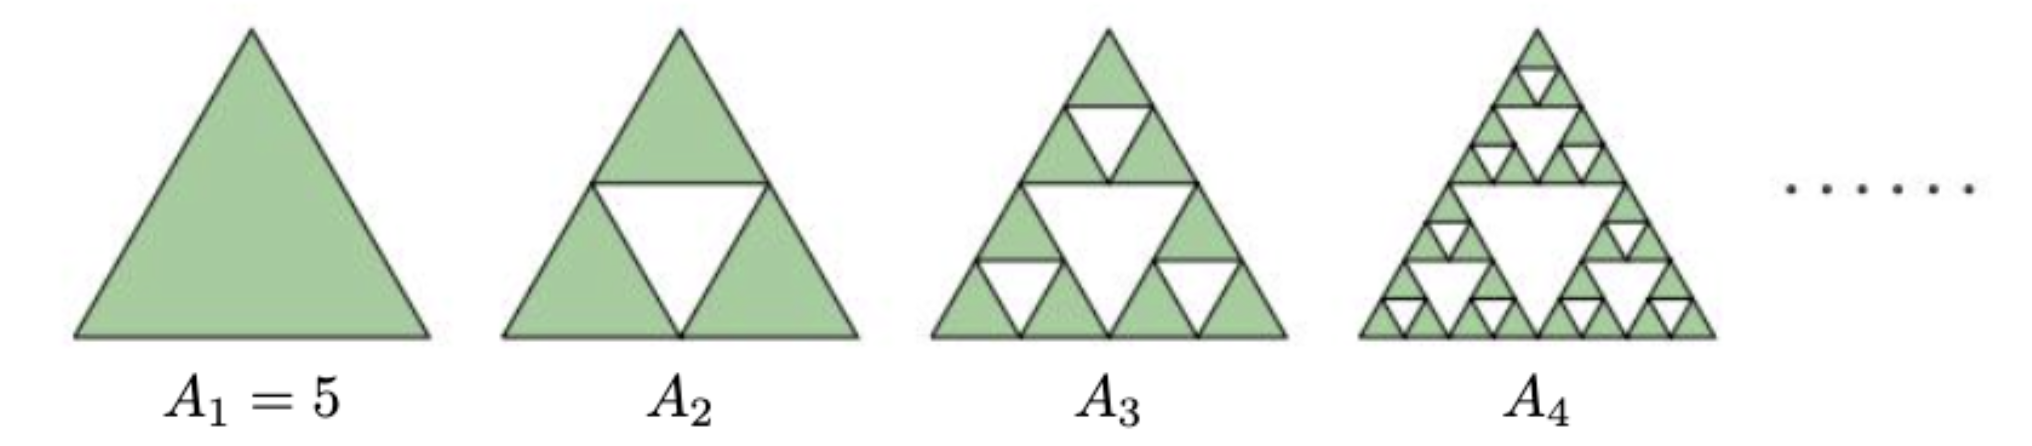
\includegraphics[width=0.8\textwidth]{media/sierpinski.png}
\end{center}

\textit{Bemerkung:} Die Figuren zeigen die ersten vier Glieder eines bekannten \textit{Fraktals}, das nach dem polnischen Mathematiker \textbf{Waclaw Franciszek Sierpinski} (1882–1969) benannt ist.

\begin{enumerate}
    \item Berechne $A_2$ und $A_3$.
    \item Bestimme die explizite Formel für $A_k$.
    \item Ab welchem $k \in \mathbb{N}$ ist $A_k$ kleiner als 0.0001?
    \item Wie viele gefärbte Dreiecke hat das $k$-te Glied bei der Konstruktion des Sierpinski-Dreiecks? Gib eine explizite Formel an.
    \item Challenge: Wie Teilaufgabe (d), jedoch sollen diesmal die weissen Dreiecke gezählt werden. \\
    \textit{Tipp:} Stelle zuerst eine rekursive Formel auf.
\end{enumerate}

        
    \end{enumerate}
\end{ueb}

\begin{ueb}
    {Programmieraufgabe}{}
    Schreiben Sie eine Python-Funktion \lstinline{isGF(liste)}, die eine Liste als Input entgegennimmt und genau dann den Wert \lstinline{True} zurückgibt, wenn die Elemente der Liste eine geometrische Folge bilden.
\end{ueb}


\clearpage
\emph{Lösungen}
\begin{enumerate}
    \item Bestimme die fehlenden Grössen dieser geometrischen Folgen (GF):
    
    \begin{center}
        \begin{tabular}{|c|c|c|c|c|c|c|}
        \hline
         & (a) & (b) & (c) & (d) & (e) & (f) \\
        \hline
        $a_1$ & 1 & 6 &  $-3$& 4 & 40 &  500\\
        \hline
        $a_n$ & 128 & 13 122 & 53 1441& 5.8564  & $-625$ & 0.16 \\
        \hline
        $n$ & 8 &  8& 12 & 5 & 4 & 6 \\
        \hline
        $q$ & 2 & 3 & $-3$ &  $1.1, -1.1$& $-2.5$ & 0.2 \\
        \hline
        $s_n$ & 255 &19 680  & 398 580 & 24.4204, 4.9724 & $-435$ & 624.96 \\
        \hline
        \end{tabular}
        \end{center}
    
    \item Anzahl der Glieder kleiner als $10^{12}$: 217
    \item Anzahl nötige Glieder:  238

    \item Berechne die Summe:
    \begin{enumerate}
        \item $\sum\limits_{k=1}^{10} \frac{5}{4}\cdot2^{k-1} = \frac{5115}{4}$
        \item $\sum\limits_{k=1}^{14} 7680 \cdot \left(\frac{1}{2}\right)^{k-1}  = 15359.0625$
        \item $\sum\limits_{k=1}^{12} -4 \cdot (-3)^{k-1}    = 531 440$
        % \item $\approx 4.42$
        % \item $\approx5173.13$
    \end{enumerate}
    
    \item Berechne die Summe:
    \begin{enumerate}
        %\item 838 861
        \item 6 560
        \item $\approx5 375 378.8$
        \item 13 107
    \end{enumerate}
    
    
    
    \item Das Sierpinski-Dreieck
    \begin{enumerate}
        \item $A_2 = 3.75$, $A_3 = 2.8125$
        \item $A_k = 5 \cdot \left( \frac{3}{4} \right)^{k-1}$
        \item $k = 39$
        \item $3^{k-1}$
        \item Die Anzahl $w_k$ der weissen Dreiecke in der $k$-te Figur ist
        $$w_k = 0 + 1 + 3 + 9 + 27 + \cdots + 3^{k-2}$$
        Mit der Formel für GR folgt $w_k = \frac{3^{k-1}-1}{2}$.
    \end{enumerate}
\end{enumerate}


















\newpage
\subsection{Die unendliche geometrische Reihe}
\subsubsection{Der Grenzwert der GR}
\begin{LA}{Einführung}{}
    Ein Baukastensatz enthält Holzwürfel. Der grösste Würfel hat eine Kantenlänge von 40 cm, die Kantenlänge des zweitgrössten misst 20 cm, die des drittgrössten 10 cm und so weiter. Ein Kind baut mit den Holzwürfeln einen Turm. Es stellt den grössten Würfel zuunterst hin, legt den zweitgrössten darauf, dann den drittgrössten und so weiter.
    \begin{enumerate}
        \item Berechnen Sie die Höhen $h_1, h_2, h_3$ und $h_{10}$ der Türme aus einem, zwei, drei und zehn Klötze.
        \item Wie viele Klötze werden benötigt, damit der Turm insgesamt einen Meter hoch wird? Wieso?
    \end{enumerate}
\end{LA}
\newpage
Die Überlegungen aus der Einführungsaufgabe lassen vermuten, dass die Glieder geometrischer Folgen $a_n = a_1 q^{n-1}$ mit $|q|<1$ für wachsende $n$ immer näher bei $0$ zu liegen kommen.
Analog wächst auch die geometrische Reihe nicht über alle Grenzen. Für wachsende $n$ nähert sich $s_n$ einer bestimmten Zahl $s$. Doch wie lässt sich $s$ aus $a_1$ und $q$ bestimmen?
Für die Summe aus $n$ Gliedern gilt:
$$s_n = a_1\cdot \frac{q^n-1}{q-1}$$
Falls nun $|q| < 1$ zum Beispiel $q=\frac{1}{2}$ ist, werden die Zahlen $q,q^2,q^3,\ldots$ immer kleiner. Die Zahl $q^{100000}$ ist dann kaum grösser als Null. Wenn $n$ gegen unendlich strebt, wird $q^n$ vernachlässigbar klein und es gilt:
$$s_n = a_1\cdot \frac{q^n-1}{q-1}   \stackrel{n\rightarrow \infty}{\longrightarrow}   s = a_1\cdot \frac{0-1}{q-1} = \frac{a_1}{1-q}$$


\begin{satz}{Unendliche geometrische Folgen und Reihen}{}
    Für die geometrische Folge
$$a_n=a_1\cdot q^{n-1}$$
gilt:
\begin{itemize}
    \item 	Falls $|q|<1$ \newline
    Die Glieder der Folge nähern sich immer mehr dem Grenzwert $0$. \newline
    Die Glieder der entsprechenden \emph{Reihe} nähern sich immer mehr dem Grenzwert
    $$ s= \frac{a_1}{1-q}$$
    \item Falls $|q|>1$ \newline
    Die Beträge der Folgenglieder wachsen über alle Grenzen. $|a_n |$ wird für wachsende $n$ unendlich gross.\newline
    Die Beträge der Reihenglieder wachsen ebenfalls über alle Grenzen. $|s_n |$ wird für wachsende $n$ unendlich gross.       
\end{itemize}
\end{satz}
\begin{definition}{Sprechweise und Notation rund um Grenzwerte}{}
Für eine geometrische Folge mit $|q|<1$ sagt man: Die Reihe \emph{konvergiert} gegen den \emph{Grenzwert} $s= \frac{a_1}{1-q}$ und man schreibt:
$$ \lim_{n \rightarrow\infty} s_n = \frac{a_1}{1-q}$$
Sprich: der \emph{Limes} für $n$ gegen unendlich von $s_n$ ist $\frac{a_1}{1-q}$

Für eine geometrische Folge mit $|q|>1$ sagt man: Die Reihe hat keinen Grenzwert. Sie \emph{divergiert}.
\end{definition}
\begin{ueb}
    {}{}

    \begin{enumerate}
        \item Ermittle den Wert der unendlichen Summe: 
        \begin{enumerate}
            \item\( 1 + \frac{1}{4} + \frac{1}{16} + \dots \)
            \item \( 5 + \frac{3}{2} + \frac{9}{20} + \dots \)
            \item \( 3 - \frac{3}{2} + \frac{3}{4} - \dots \)
           % \item \( 1 - \frac{2}{3} + \frac{4}{9} - \dots \)
            \item \( 2 + \sqrt{2} + 1 + \dots \)
            % \item \( 8 + 4\sqrt{3} + 6 + \dots \)
        \end{enumerate}
       
        \item Der Schlangenweg von $P$ nach $Q$ setzt sich aus unendlich vielen Halbkreisbögen zusammen, deren Radien eine GF mit $q = \frac{1}{2}$ bilden. Ist der Schlangenweg oder der Halbkreisweg von $P$ nach $Q$ kürzer?
        
       
        
        
        \begin{center}
            % 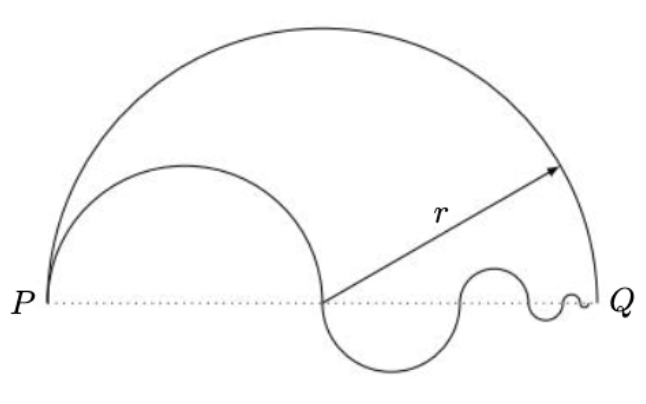
\includegraphics[width = 0.5\textwidth]{media/Schlangenweg.png}
            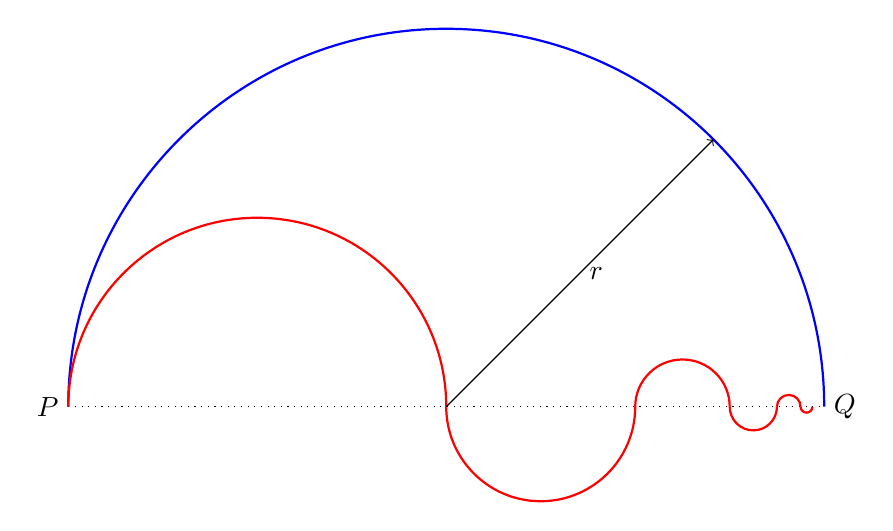
\begin{tikzpicture}[scale=0.3]
                % Achsen
                \draw[dotted] (-16,0) -- (16,0);
                
                % Kreise und Wellen
                \draw[blue, thick] (-16,0) arc[start angle=180, end angle=0, radius=16cm];
                \draw[red, thick] (-16,0) arc[start angle=180, end angle=0, radius=8cm];
                \draw[red, thick] (0,0) arc[start angle=180, end angle=360, radius=4cm];
                \draw[red, thick] (8,0) arc[start angle=180, end angle=0, radius=2cm];
                \draw[red, thick] (12,0) arc[start angle=180, end angle=360, radius=1cm];
                \draw[red, thick] (14,0) arc[start angle=180, end angle=0, radius=0.5cm];
                \draw[red, thick] (15,0) arc[start angle=180, end angle=360, radius=0.25cm];




                % \draw (0,0) arc[start angle=180, end angle=0, radius=2.5cm];
                % \draw (4,0) .. controls (5,-0.5) and (5.5,0.5) .. (6,0)
                %             .. controls (6.5,-0.5) and (7,0.5) .. (7.5,0)
                %             .. controls (7.75,-0.2) and (8,0.2) .. (8.2,0);
                
                % Radiuslinie
                \draw[->] (0,0) -- (45:16) node[midway, right] {$r$};
                
                % Punktebeschriftung
                \node[left] at (-16,0) {$P$};
                \node[right] at (16,0) {$Q$};
                
            \end{tikzpicture}
        \end{center}




        \item Ein Spiralförmiger Weg beginnt im Ursprung und besteht aus Strecken, deren Längen eine GF bilden. Wie lang ist der unendlich fortgesetzte Weg und wo liegt der Zielpunkt $Z$ dieses Spiralförmigen Weges?
        \begin{center}
            %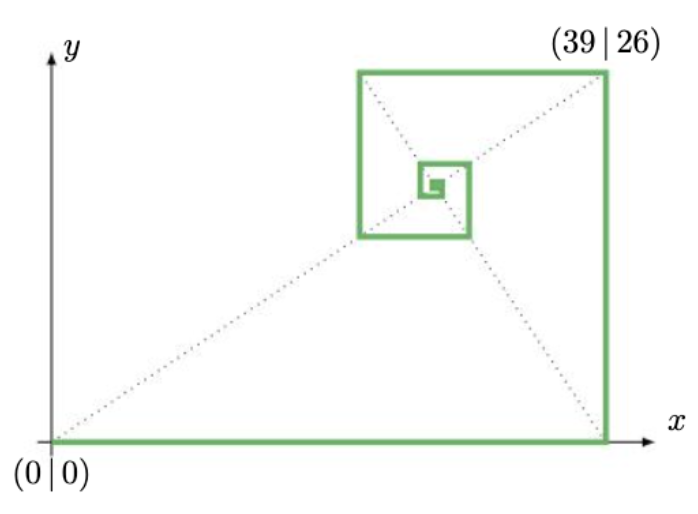
\includegraphics[width = 0.5\textwidth]{media/Spiralenweg.png}
            \begin{tikzpicture}[scale=0.5]
                % Achsen
                \draw[->] (-1,0) -- (10,0) node[right] {$x$};
                \draw[->] (0,-1) -- (0,7) node[above] {$y$};
                
                % Spiralenerstellung mit den Fibonacci-Zahlen
                \draw[thick,red] (0,0) -- (9,0) -- (9,6) -- (5,6) -- (5,10/3)
                    -- (6.77,10/3) -- (6.77,4.51) -- (5.99,4.51) -- (5.99,3.99) -- (6.33,3.99)
                     -- (6.33, 4.22);
                
                % Diagonalen
                \draw[dotted] (0,0) -- (9,6);
                \draw[dotted] (9,0) -- (5,6);
                % \draw[dotted] (8,5) -- (3,2);
                % \draw[dotted] (3,2) -- (4,2.5);
                
                % Punktebeschriftung
                \node[below left] at (0,0) {(0, 0)};
                \node[above right] at (9,6) {(39, 26)};
                
            \end{tikzpicture}
        \end{center}
        

        \item Eine unendliche geometrische Reihe beginnt mit 
        \[
        (x - 3) + \frac{1}{x - 3} + \dots \quad (x \neq 3).
        \]
        
        \begin{enumerate}
            \item Für welche Werte von \( x \) konvergiert die Reihe?
            \item Zeige, dass in diesem Fall für die Summe gilt: 
            \[
            s = \frac{(x - 3)^3}{(x - 2)(x - 4)}.
            \]
            \item Für welchen Wert von \( x \) gilt, dass \( s = x + 2 \)?
        \end{enumerate}
    \end{enumerate}
\end{ueb}

\clearpage
\emph{Lösungen}
\begin{enumerate}
    \item Ermittle den Wert der unendlichen Summe: 
    \begin{enumerate}
        \item\(  \frac{4}{3}  \)
        \item \( \frac{50}{7} \)
        \item \( 2\)
        %\item \( \frac{3}{5} \)
        \item \( 4 + 2\sqrt{2} \)
        %\item \( 32 + 16\sqrt{3} \)
    \end{enumerate}
    \item Beide Wege sind gleich lang :) .
    \item Länge 117, Endpunkt $Z=(27, 18)$
    
    \item Eine unendliche geometrische Reihe beginnt mit 
    \(
    (x - 3) + \frac{1}{x - 3} + \dots \quad (x \neq 3).
    \)
    
    \begin{enumerate}
        \item $x<4$ oder $x<2$.
        \item \dots
        \item \( x \approx 4.10\)
    \end{enumerate}
\end{enumerate}




























\newpage
\subsubsection{Dezimalbruchdarstellung rationaler und irrationaler Zahlen}
Bereits in der ersten Klasse haben Sie gelernt, dass Zahlen mit einer unendlichen, periodischen Dezimaldarstellung einem gewöhnlichen Bruch entsprechen. Allerdings konnten wir es damals nicht begründen. Heute werden Sie sehen, dass konvergente unendliche geometrische Reihen der Schlüssel für die Umwandlung solcher Zahlen in Brüche sind. Betrachten Sie dazu folgende Beispiele:
\begin{bsp}{Umwandlung von periodischen Zahlen in Brüche}{}
    \vspace*{15cm}
%    \begin{itemize}
%     \item Mit Periode, die aus einer Ziffer besteht:
%     \begin{align*} 0.\overline{4} 
%         &= 0.4444\cdots = 0.4 + 0.04 + 0.004 + \cdots = \frac{4}{10} + \frac{4}{100} +\frac{4}{1000} +\cdots = \\
%                                     &= \frac{4}{10} \left( 1+\frac{1}{10} + \frac{1}{100} + \cdots \right) = \frac{4}{10}\cdot \frac{1}{1-\frac{1}{10}}=\frac{4}{9}
%         \end{align*}

%     \item  Mit Periode, die aus zwei Ziffern besteht:
%     \begin{align*} 0.\overline{37} &= 0.373737\cdots = 0.37 + 0.0037 + 0.000037 + \cdots = \frac{37}{100} + \frac{37}{10000} +\frac{37}{1000000} +\cdots = \\
%                                     &= \frac{37}{100} \left( 1+\frac{1}{100} + \frac{1}{10000} + \cdots \right) = \frac{37}{100}\cdot \frac{1}{1-\frac{1}{100}}=\frac{37}{99}
%         \end{align*}
%     \item  Wenn die Periode nicht gleich nach dem Dezimalpunkt steht:
%         \begin{align*} 0.135\overline{37} = \frac{135}{1000} + \frac{37}{10^5}\left( 1+\frac{1}{100} + \frac{1}{10000} + \cdots \right) = \frac{135}{1000} + \frac{37}{10^5} \cdot \frac{1}{1-\frac{1}{100}}=\frac{6701}{49500}
%             \end{align*} 
%     \end{itemize}
\end{bsp}

\clearpage

\begin{ueb}
    {}{}
    \begin{enumerate}
        % \item Verwandeln Sie die folgenden Zahlen in Brüche
        % \begin{tasks}(3)
        %     \task $0.\overline{7}$
        %     \task $0.\overline{54}$
        %     \task $0.\overline{612}$
        %     \task $2.\overline{04}$
        %     \task $0.63\overline{123}$
        %     \task $1.00\overline{35}$
        % \end{tasks}
        \item  Verwandle den periodischen Dezimalbruch in einen gewöhnlichen Bruch. (Überprüfen Sie das Resultat mit dem Taschenrechner)

        \begin{enumerate}
            %\item \( 0.\overline{5} \)
            %\item \( 0.\overline{54} \)
            \item \( 0.\overline{543} \)
            %\item \( 0.1\overline{3} \)
            \item \( 0.25\overline{7} \)
            \item \( 0.4\overline{81} \)
        \end{enumerate}
        
        \item Aus den Überlegungen oben folgt, dass jede Zahl mit einer endlichen oder periodischen Dezimaldarstellung einem Bruch entspricht. Es gilt auch die \emph{Umkehrung}: Die Dezimaldarstellung eines Bruchs ist immer endlich oder periodisch. Die folgenden Aufgaben sollen Ihnen helfen zu verstehen, wieso das so ist.
        \begin{enumerate}
            \item Finden Sie die Dezimaldarstellung von $\frac{1}{7}$, indem Sie schriftlich dividieren:
            \begin{align*}
                &1.00000 : 7 = 0.1\ldots \\
                &10 \\
                &\phantom{1}30
            \end{align*}
            \item 	Wann beginnt sich die Dezimaldarstellung zu wiederholen? Wie viele verschiedene Reste kann es bei einer Division durch eine ganze Zahl $n$ geben?
            \item 	Wieso ist die Dezimaldarstellung von $\frac{1}{n}$ endlich oder periodisch? Wie lang kann die Periode sein?
        \end{enumerate}
        
    \end{enumerate}
\end{ueb}

% \emph{Lösungen}
% \begin{enumerate}

%     \item  Verwandle den periodischen Dezimalbruch in einen gewöhnlichen Bruch.

%     \begin{enumerate}
%         %\item \( \frac{5}{9}  \)
%         %\item \( \frac{6}{11} \)
%         \item \( \frac{181}{333}  \)
%         %\item \(\frac{2}{15}  \)
%         \item \( \frac{58}{225}  \)
%         \item \( \frac{53}{110}  \)
%     \end{enumerate}
    
%     \item \dots 
%     \end{enumerate}

